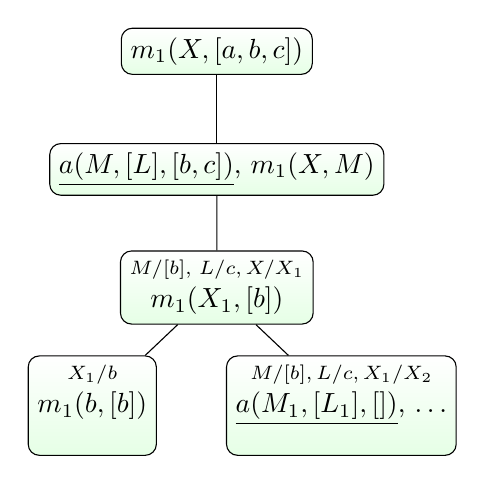
\begin{tikzpicture}[sibling distance=9em, align=center,
  every node/.style = {shape=rectangle, rounded corners,
    draw, align=center,
    top color=white, bottom color=green!10}]]
  \node {$m_1(X,[a,b,c])$}
    child { node {\underline{$a(M, [L], [b,c])$}, $m_1(X, M)$}
      child { node {\scriptsize $M/[b]$, $L/c, X/X_1$\\$m_1(X_1, [b])$}
        child { node {\scriptsize $X_1/b$\\ $m_1(b, [b])$\\$\blacksquare$}}
        child { node {\scriptsize $M/[b], L/c, X_1/X_2$\\\underline{$a(M_1, [L_1], [])$}, $\ldots$\\$\square$}}
      }
    };
\end{tikzpicture}